%%%%%%%%%%%%%%%%%%%%%%%%%%%%%%%%%%%%%%%%%
%% Appendix section
% Set-up the section.
%\newpage
\appendix
\setcounter{table}{0}
\renewcommand{\thetable}{A\arabic{table}}
\setcounter{figure}{0}
\renewcommand{\thefigure}{A\arabic{figure}}

% Start appendix
\section{Appendix}
\label{appendix}
This project used data which are fully public, and computational tools which are fully open-source.
%As such, all code and data involved in this project are available at this project's Github repository, available at \url{https://github.com/shoganhennessy/state-faculty-composition}.
%They may be used for replication, or as the basis for further work, as needed.
Any comments or suggestions may be sent to me at \href{mailto:seh325@cornell.edu}{\nolinkurl{seh325@cornell.edu}}, or raised as an issue on the Github project.

A number of statistical packages, for the R language \citep{R2023}, made the empirical analysis for this paper possible.
\begin{itemize}
    \item \textit{Tidyverse} \citep{tidyverse} collected tools for data analysis in the R language.
    \item \textit{GRF} \citep{athey2019generalized,grf} compiled forest computational tools for the R language.
    \item \textit{Stargazer} \citep{stargazer} provided methods to efficiently convert empirical results into presentable output in \LaTeX.
\end{itemize}

\subsection{Additional MR Results}

\begin{table}[H]
    \singlespacing
    \small
    \centering
    \caption{First Stage Estimates, for Effect of EA score on Education in HRS Data.}
    \makebox[\textwidth][c]{\input{sections/tables/firststage-reg.tex}}
    \label{tab:firststage-reg}
    \justify
    \footnotesize
    \textbf{Note}:
    This table shows OLS results of the first stage, $D_i = \alpha_i + \beta_i Z_i + \varepsilon_i$.
\end{table}

\begin{table}[H]
    \singlespacing
    \small
    \centering
    \caption{Reduced Form Estimates, for Effect of EA score on Annual Earnings in HRS Data.}
    \makebox[\textwidth][c]{\input{sections/tables/reducedform-reg.tex}}
    \label{tab:reducedform-reg}
    \justify
    \footnotesize
    \textbf{Note}:
    This table shows OLS results of the reduced form, $Y_i = \alpha_i + \beta_i Z_i + \varepsilon_i$.
\end{table}

\subsection{Compliance Scores}
\begin{proof}
    \label{proof:complierscore}
    \citet[Lemma~3.1]{abadie2003semiparametric} shows that complier score, always-taker score, and never-taker score are all identified, in expectation and in conditional expectation.
    The derivation is re-presented here, to elucidate the reasoning.

    Complier score,
    \begin{align*}
        \Probgiven{D_i(1) > D_i(0)}{\mat X_i}
            &= 1 - \Probgiven{D_i(1) = D_i(0) = 0}{\mat X_i} - \Probgiven{D_i(1) = D_i(0) = 1}{\mat X_i} \\
            \text{(by independence of $Z_i$)} &=
                1 - \Probgiven{D_i(1) = D_i(0) = 0}{\mat X_i, Z_i = 1} - \Probgiven{D_i(1) = D_i(0) = 1}{\mat X_i, Z_i = 0} \\
            \text{(by monotonicity)} &=
                1 - \Probgiven{D_i = 0}{\mat X_i, Z_i = 1} - \Probgiven{D_i = 1}{\mat X_i, Z_i = 0} \\
            &= \Probgiven{D_i = 1}{\mat X_i, Z_i = 1} - \Probgiven{D_i = 1}{\mat X_i, Z_i = 0} \\
            &= \Egiven{D_i}{\mat X_i, Z_i = 1} - \Egiven{D_i}{\mat X_i, Z_i = 0} \\
    \end{align*}
    By similar reasoning, for always-takers,
    \[ \Probgiven{D_i(1) = D_i(0) = 1}{\mat X_i} = \Egiven{D_i}{\mat X_i, Z_i = 0} \]
    And for never-takers,
    \[ \Probgiven{D_i(1) = D_i(0) = 0}{\mat X_i} = 1 - \Egiven{D_i}{\mat X_i, Z_i = 1}. \]
\end{proof}

\subsection{Connection Between Causal Mediation Effect and LATE}
\label{sec:acme-late}
\cite{imai2010identification} focuses on decomposing the total effect into the causal mediation and direct effects.
To define the average causal mediation effect, this corresponds to the effect on $Y_i$ by manipulation of $D_i$, while holding $Z_i$ constant.
\[ \E{ \Egiven[Z]{ Y_i(z, D_i(1)) - Y_i(z, D_i(0)) }{Z_i = z}} \]
Now we can expand the average causal mediation effect, to show it is the product of first stage effect and LATE.
\begin{align*}
    &\E{ \Egiven[Z]{ Y_i(z, D_i(1)) - Y_i(z, D_i(0)) }{Z_i = z}} \\
    =& 
    \Prob{D_i(1) = 1, D_i(0) = 0}
    \Egiven{ \Egiven[Z]{ Y_i(z, 1) - Y_i(z, 0) }{Z_i = z}}{
        D_i(1) = 1, D_i(0) = 0} \\
    & + \Prob{D_i(1) = D_i(0) = 1}
    \Egiven{ \Egiven[Z]{ Y_i(z, 1) - Y_i(z, 1) }{Z_i = z}}{
        D_i(1) = D_i(0) = 1} \\
    & + \Prob{D_i(1) = D_i(0) = 0}
    \Egiven{ \Egiven[Z]{ Y_i(z, 0) - Y_i(z, 0) }{Z_i = z}}{
        D_i(1) = D_i(0) = 0} \\
    =& \Prob{D_i(1) = 1, D_i(0) = 0}
    \Egiven{ \Egiven[Z]{ Y_i(z, 1) - Y_i(z, 0) }{Z_i = z}}{
        D_i(1) = 1, D_i(0) = 0} \\
    =& \E{D_i(1) - D_i(0)}
    \Egiven{ \Egiven[Z]{ Y_i(z, 1) - Y_i(z, 0) }{Z_i = z}}{
        D_i(1) = 1, D_i(0) = 0} \\
    =& \text{ first-stage} \times \text{LATE} \\
\end{align*}
The first equality comes from assuming no defiers, and compliers with $D_i(1) = 1, D_i(0) = 0$ being the only individuals with $Y_i(z, D_i(1)) \neq Y_i(z, D_i(0))$ for $z = 0,1$.
Note that this is an example of the \textit{front-door criterion} identification approach \citep{pearl2003direct}, where the LATE is not identified on its own without further assumptions.

\subsection{Wald Estimand Decomposition}
\begin{proof}[Proof of~\autoref{theorem:nonidentified}]
    \label{proof:nonidentified}
    This sequence follows the set-up first presented in \citet[Section~2]{imbens1994identification}, but now does not assume exclusion.
    \begin{align*}
        & &\Egiven{Y_i}{Z_i = 1} - \Egiven{Y_i}{Z_i = 0} \\
        &=& \Egiven{D_i(1) Y_i(1,1) + (1 - D_i(1)) Y_i(1,0)}{Z_i = 1} \\
        &&+ \Egiven{D_i(0) Y_i(0,1) + (1 - D_i(0)) Y_i(0,0)}{Z_i = 0} \\
            %\text{by independence of POs w.r.t. $Z_i$}
        &=& \E{D_i(1) \left(Y_i(1,1) - Y_i(1,0)\right)
                - D_i(0) \left(Y_i(0,1) - Y_i(0,0)\right)
                + \left(Y_i(1,0) - Y_i(0,0)\right)} \\
        &=& \Prob{D_i(1) = 1, D_i(0) = 0}
            \Egiven{Y_i(1,1) - Y_i(0,0)}{D_i(1) = 1, D_i(0) = 0} \\
            &&+ \Prob{D_i(1) = D_i(0) = 1}
                \Egiven{Y_i(1,1) - Y_i(0,1)}{D_i(1) = D_i(0) = 1} \\
            &&+ \Prob{D_i(1) = D_i(0) = 0}
                \Egiven{Y_i(1,0) - Y_i(0,0)}{D_i(1) = D_i(0) = 0}
    \end{align*}
    Decompose the combined effect of  $Z,D \to Y$ among compliers into two components: (1) the LATE (effect $D \to Y$), and (2) an irregularly weighted left-over term (direct effect $Z \to Y$).
    \begin{align*}
        &\Egiven{Y_i(1,1) - Y_i(0,0)}{D_i(1) = 1, D_i(0) = 0} \\
        &=
        \Egiven{ Z_i \left(Y_i(1, 1) - Y_i(1, 0) \right)
            + (1 - Z_i) \left(Y_i(0, 1) - Y_i(0, 0) \right)}{
                D_i(1) = 1, D_i(0) = 0} \\
        &\;\;\;\; + \Egiven{ Z_i \left(Y_i(1, 0) - Y_i(0, 0) \right)
            + (1 - Z_i) \left(Y_i(1, 1) - Y_i(0, 1) \right)}{
                D_i(1) = 1, D_i(0) = 0}
    \end{align*}
    The second term is \textit{irregularly weighted} as the weights on the POs do not sum in expectation, and has no further simplified form

    Together, this yields the reduced form effect as a weighted sum of local treatment and direct effects: 
    \begin{align*}
        &\Egiven{Y_i}{Z_i = 1} - \Egiven{Y_i}{Z_i = 0} \\
        &= 
        \underbrace{\Prob{D_i(1) = 1, D_i(0) = 0}}_{\text{Complier score}} \\
        & \;\;\;\; \;\;\;\; \times
        \underbrace{\Egiven{ Z_i \left(Y_i(1, 1) - Y_i(1, 0) \right)
            + (1 - Z_i) \left(Y_i(0, 1) - Y_i(0, 0) \right) }{
                D_i(1) = 1, D_i(0) = 0}}_{
                    \text{LATE, effect of } D \to Y \text{ among compliers}} \\
        & \;\;\;\; +
        \underbrace{\Prob{D_i(1) = 1, D_i(0) = 0}}_{\text{Complier score}} \\
        & \;\;\;\; \;\;\;\; \times
        \underbrace{\Egiven{Z_i \left(Y_i(1, 0) - Y_i(0, 0) \right)
            + (1 - Z_i) \left(Y_i(1, 1) - Y_i(0, 1) \right)}{
                D_i(1) = 1, D_i(0) = 0}}_{
                    \text{Left-over ADE term, effect of } Z \to Y \text{ among compliers}} \\
        & \;\;\;\; + 
        \underbrace{\Prob{D_i(1) = D_i(0) = 1}}_{\text{Always-taker score}}
        \times
        \underbrace{\Egiven{Y_i(1,1) - Y_i(0,1)}{D_i(1) = D_i(1) = 1}}_{
                \text{LADE, effect of } Z \to Y \text{ among always-takers}
            } \\
        & \;\;\;\; + \underbrace{\Prob{D_i(1) = D_i(0) = 0}}_{\text{Never-taker score}}
        \times
        \underbrace{\Egiven{Y_i(1,0) - Y_i(0,0)}{D_i(1) = D_i(1) = 0}}_{
                \text{LADE, effect of } Z \to Y \text{ among never-takers}
            }
    \end{align*}
    Recall that the complier score is identified: $\Prob{D_i(1) = D_i(0) = 1} = \Egiven{D_i}{Z_i = 1} - \Egiven{D_i}{Z_i = 0}$.
    Dividing both sides by the complier score yields the theorem.
    \begin{align*}
        &\frac{ \Egiven{Y_i}{Z_i = 1} - \Egiven{Y_i}{Z_i = 0}}{
            \Egiven{D_i}{Z_i = 1} - \Egiven{D_i}{Z_i = 0}} \\
        &= \Egiven{ Z_i \left(Y_i(1, 1) - Y_i(1, 0) \right)
            + (1 - Z_i) \left(Y_i(0, 1) - Y_i(0, 0) \right)}{
                D_i(1) = 1, D_i(0) = 0} \\
        &+ \Egiven{ Z_i \left(Y_i(1, 0) - Y_i(0, 0) \right)
            + (1 - Z_i) \left(Y_i(1, 1) - Y_i(0, 1) \right)}{
                D_i(1) = 1, D_i(0) = 0} \\
        &+ \frac{\Prob{D_i(1) = D_i(0) = 1}}{\Prob{D_i(1) = 1, D_i(0) = 0}}
            \Egiven{Y_i(1,1) - Y_i(0,1)}{D_i(1) = D_i(0) = 1} \\
        &+ \frac{\Prob{D_i(1) = D_i(0) = 0}}{\Prob{D_i(1) = 1, D_i(0) = 0}}
            \Egiven{Y_i(1,0) - Y_i(0,0)}{D_i(1) = D_i(0) = 0}
    \end{align*}
\end{proof}

\subsection{Identification via CCI}
\label{sec:cci-identification}

The ATE depends only on the first moments of the potential earnings states.
\[ \E{ Z_i \left(Y_i(1, 1) - Y_i(1, 0) \right)
    + (1 - Z_i) \left(Y_i(0, 1) - Y_i(0, 0) \right)} \]
$Z_i$ is indepedent of POs, so it suffices to identify each $\E{ Y_i(z, d) }$ for $z,d = 0,1$ to compose the mechanism effect --- or subgroup versions.

While each unconditional potential outcome is not identified without further assumptions, they are identified for differing compliance groups already.
To see this, notice that $Y_i = Y_i(1,1)$ is realised by always--takers and compliers who receive $Z_i = 1$.
So that the conditional expectation of earnings data among $Z_i = D_i = 1$ reveals the potential earnings $Y_i(1,1)$ among this subgroup.
\[ \Egiven{ Y_i }{ \vec X_i, Z_i = D_i = 1}
= \underbrace{\Egiven{ Y_i(1,1) }{ \vec X_i, D_i(1) = 1}}_{
    Y_i(1,1) \text{ among compliers and always--takers}
} \]
Similarly, $Y_i = Y_i(0,0)$ is revealed by never--takers and compliers who receive $Z_i = 0$.
\[ \Egiven{ Y_i }{ \vec X_i, Z_i = D_i = 0}
= \underbrace{\Egiven{ Y_i(0,0) }{ \vec X_i, D_i(0) = 0}}_{
    Y_i(0,0) \text{ among compliers and never--takers}
} \]

The observation $Z_i = 0, D_i = 1$ reveals that $i$ is an always--taker, and their potential earnings $Y_i(0, 1)$.
\[ \Egiven{ Y_i }{ \vec X_i, Z_i = 0, D_i = 1}
= \underbrace{\Egiven{ Y_i(0,1) }{ \vec X_i, D_i(0) = D_i(1) = 1}}_{
    Y_i(0,1) \text{ among always--takers}
} \]
Conversely, $Z_i = 1, D_i = 0$ reveals that $i$ is a never--taker, and their potential earnings $Y_i(1, 0)$.
\[ \Egiven{ Y_i }{ \vec X_i, Z_i = 1, D_i = 0}
= \underbrace{\Egiven{ Y_i(1,0) }{ \vec X_i, D_i(0) = D_i(1) = 0}}_{
    Y_i(1,0) \text{ among never--takers}
} \]

Point identification may be achieved under the assumption that composing the four above terms is equivalent to their unconditional expectation (i.e., CCI \ref{definition:cci}).
CCI (\ref{definition:cci}) assumes earnings vary between compliers, always--takers, and never--takers only through pre-determined characteristics $\vec X_i$.
In essence, POs do not on average differ thanks to unobserved factors.
The assumption is a slightly stronger version of that first presented by \citet[Assumption~3]{angrist2010extrapolate}.
%A sufficient condition for CCI is that mean potential earnings are a function of $\vec X_i$, $\Egiven{Y_i(Z, D)}{\vec X_i} = g(\vec X_i)$.
In application, individuals who would attend higher education with a higher EA score have the same average earnings as those who never- or always-attend, after accounting for characteristics $\vec X_i$.
This means $\vec X_i$ must contain important information on labour market determinants, such as gender, age at measured income, and any other determinant that systematically affects later life earnings.

\begin{figure}[h!]
    \centering
    \caption{Conditional Compliance Ignorability (CCI) Across Compliance Regions.}
    \label{fig:ignorability-compliance-extrapolate}
    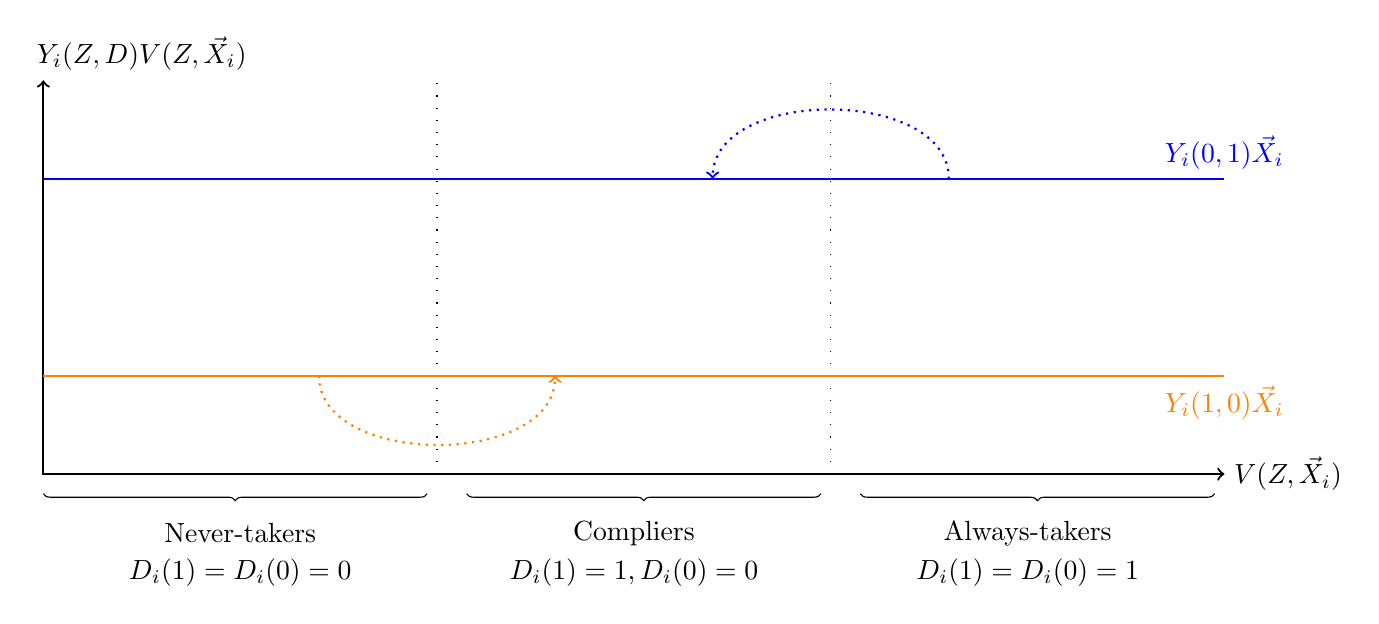
\begin{tikzpicture}[scale=5]
        % Axis
        \draw[thick,<->] (0,1)--(0,0)--(3,0);
        % Labels
        \node [above] at (0.25,1) {$\Egiven{Y_i(Z,D)}{V(Z, \vec{X}_i)}$};
        \node [right] at (3,0) {$V(Z, \vec{X}_i)$};
        % Draw the compliance regions
        \draw[decorate, decoration = {brace}] (0.975,-0.05) --  (0,-0.05);
        \node at (0.5,-0.15) {Never-takers};
        \node at (0.5,-0.25) {$D_i(1)=D_i(0)=0$};
        \draw[loosely dotted] (1,0)--(1,1);
        \draw[decorate, decoration = {brace}] (1.975,-0.05) --  (1.075,-0.05);
        \node at (1.5,-0.15) {Compliers};
        \node at (1.5,-0.25) {$D_i(1)=1, D_i(0)=0$};
        \draw[loosely dotted] (2,0)--(2,1);
        \draw[decorate, decoration = {brace}] (2.975,-0.05) --  (2.075,-0.05);
        \node  at (2.5,-0.15) {Always-takers};
        \node  at (2.5,-0.25) {$D_i(1)=D_i(0)=1$};
        % Draw Y_i(0, 1)
        \draw[thick,blue] (0,0.75)--(3,0.75);
        \node [above,blue] at (3,0.75) {$\Egiven{Y_i(0,1)}{\vec{X}_i}$};
        % Draw extrapolation of Y_i(0, 1)
        \draw[thick,dotted,->,blue] (2.3,0.75) to [out=90,in=90] (1.7,0.75);
        % Draw Y_i(0, 1)
        \draw[thick,orange] (0,0.25)--(3,0.25);
        \node [below,orange] at (3,0.25) {$\Egiven{Y_i(1,0)}{\vec{X}_i}$};
        % Draw extrapolation of Y_i(1, 1)
        \draw[thick,dotted,->,orange] (0.7,0.25) to [out=-90,in=-90] (1.3,0.25);
    \end{tikzpicture}
    \justify
    \footnotesize
    \textbf{Note}:
    The figure shows how the CCI assumption \ref{assumption:compliance-ignorability} works.
    The $x$-axis partitions compliers from non-compliers --- i.e., $V(.;.)$ is the theoretical latent-index implied by the IV assumptions \citep{vytlacil2002independence}. 
    The dotted blue arrow represents that $\Egiven{Y_i(0,1)}{\vec{X}_i}$ can be extrapolated out of the always-takers group to compliers.
    The dotted orange arrow represents that $\Egiven{Y_i(1,0)}{\vec{X}_i}$ can be extrapolated out of the never-takers group to compliers.
\end{figure}

This allows for extrapolation of conditional average earnings across compliance groups.
$Y_i(0, 1)$ is only observed among always--takers, so to identify the unconditional expectation, we must extrapolate $\Egiven{Y_i(0,1)}{\vec X_i}$ from $\vec X_i$ values for those with $Z_i = 0, D_i = 1$ to all values of $\vec X_i$.
\autoref{fig:ignorability-compliance-extrapolate} shows this assumption for $\Egiven{Y_i(0,1)}{\vec X_i}$, and \autoref{fig:ignorability-compliance-sum} the corresponding for $\Egiven{Y_i(1,1)}{\vec X_i}$.

\begin{figure}[h!]
    \centering
    \caption{Conditional Compliance Ignorability (CCI) Across Compliance Regions.}
    \label{fig:ignorability-compliance-sum}
    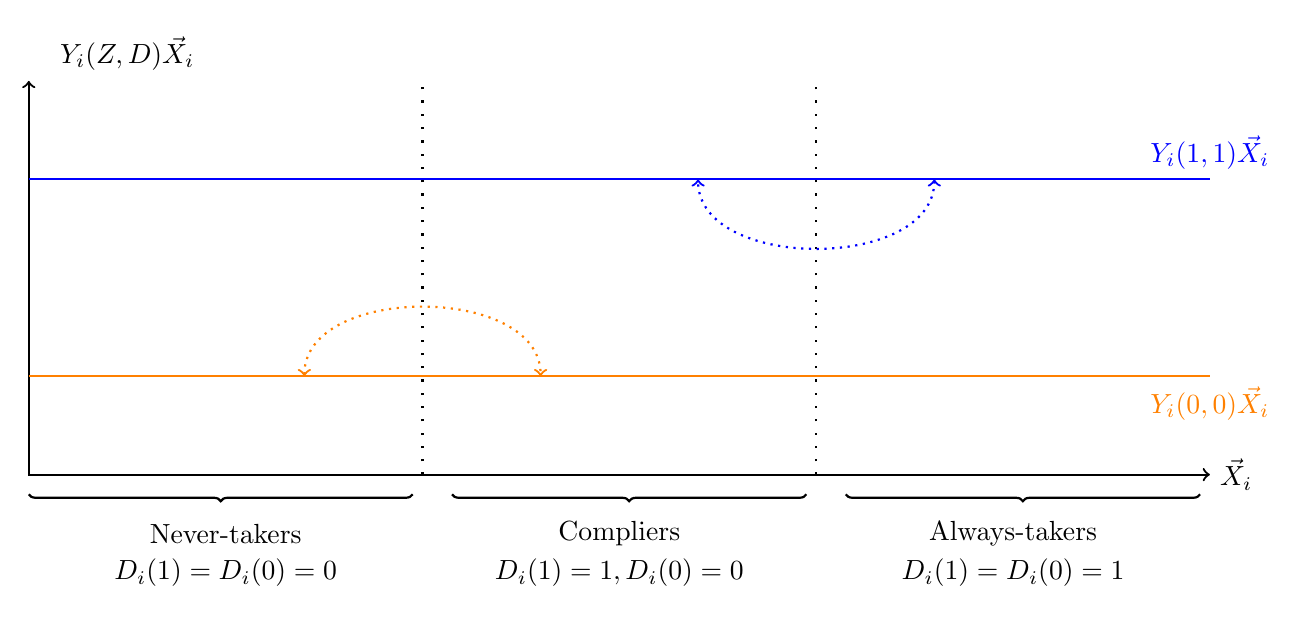
\begin{tikzpicture}[thick,scale=5]
        % Axis
        \draw[thick,<->] (0,1)--(0,0)--(3,0);
        % Labels
        \node [above] at (0.25,1) {$\Egiven{Y_i(Z,D)}{\vec{X}_i}$};
        \node [right] at (3,0) {$\vec{X}_i$};
        % Draw the compliance regions
        \draw[decorate, decoration = {brace}] (0.975,-0.05) --  (0,-0.05);
        \node at (0.5,-0.15) {Never-takers};
        \node at (0.5,-0.25) {$D_i(1)=D_i(0)=0$};
        \draw[loosely dotted] (1,0)--(1,1);
        \draw[decorate, decoration = {brace}] (1.975,-0.05) --  (1.075,-0.05);
        \node at (1.5,-0.15) {Compliers};
        \node at (1.5,-0.25) {$D_i(1)=1, D_i(0)=0$};
        \draw[loosely dotted] (2,0)--(2,1);
        \draw[decorate, decoration = {brace}] (2.975,-0.05) --  (2.075,-0.05);
        \node  at (2.5,-0.15) {Always-takers};
        \node  at (2.5,-0.25) {$D_i(1)=D_i(0)=1$};
        % Draw Y_i(1, 1)
        \draw[thick,blue] (0,0.75)--(3,0.75);
        \node [above,blue] at (3,0.75) {$\Egiven{Y_i(1,1)}{\vec{X}_i}$};
        % Draw extrapolation of Y_i(1, 1)
        \draw[thick,dotted,<->,blue] (2.3,0.75) to [out=-90,in=-90] (1.7,0.75);
        % Draw Y_i(0, 0)
        \draw[thick,orange] (0,0.25)--(3,0.25);
        \node [below,orange] at (3,0.25) {$\Egiven{Y_i(0,0)}{\vec{X}_i}$};
        % Draw extrapolation of Y_i(0, 0)
        \draw[thick,dotted,<->,orange] (0.7,0.25) to [out=90,in=90] (1.3,0.25);
    \end{tikzpicture}
    \justify
    \footnotesize
    \textbf{Note}:
    The figure shows how the CCI assumption \ref{assumption:compliance-ignorability} works.
    The dotted blue arrow represents that $\Egiven{Y_i(1,1)}{\vec{X}_i}$ is observed as the sum of outcomes among the always-takers and compliers.
    The dotted orange arrow represents that $\Egiven{Y_i(1,0)}{\vec{X}_i}$ is observed as the sum of outcomes among the always-takers and compliers.
\end{figure}

Under the CCI assumption, the conditional mechanism effect is identified.
\begin{align*}
    & \Egiven{ Z_i \left(Y_i(1, 1) - Y_i(1, 0) \right)
    + (1 - Z_i) \left(Y_i(0, 1) - Y_i(0, 0) \right)}{\vec X_i} \\
    =& \Probgiven{Z_i = 1}{\vec X_i} \left(
        \Egiven{ Y_i }{ \vec X_i, Z_i = D_i = 1}
            - \Egiven{ Y_i }{ \vec X_i, Z_i = 1, D_i = 0} \right) \\
    &+ \Probgiven{Z_i = 0}{\vec X_i} \left(
        \Egiven{ Y_i }{ \vec X_i, Z_i = 0, D_i = 1}
            - \Egiven{ Y_i }{ \vec X_i, Z_i = D_i = 0} \right)
\end{align*}
The unconditional average mechanism effect comes from integrating across the entire distribution $\vec X_i$ \citep{frolich2007nonparametric}, giving a matching--type identification.
\begin{align*}
    & \E{ Y_i(., 1) - Y_i(., 0) } \\
    &=\E[\vec X_i]{ \Egiven{ Y_i(., 1) - Y_i(., 0) }{\vec X_i}} \\
    &= \E[\vec X_i]{ \Egiven{ Z_i \left(Y_i(1, 1) - Y_i(1, 0) \right)
    + (1 - Z_i) \left(Y_i(0, 1) - Y_i(0, 0) \right)}{\vec X_i}} \\
    &= \Prob{Z_i = 1} \E[\vec X_i]{
        \Egiven{ Y_i }{ \vec X_i, Z_i = D_i = 1}
            - \Egiven{ Y_i }{ \vec X_i, Z_i = 1, D_i = 0} } \\
    &\;\;\;\; + \Prob{Z_i = 0} \E[\vec X_i]{
        \Egiven{ Y_i }{ \vec X_i, Z_i = 0, D_i = 1}
            - \Egiven{ Y_i }{ \vec X_i, Z_i = D_i = 0}}
\end{align*}

The equation for average direct effect is less simple, since $D_i$ is not independent of potential outcomes $Y_i(Z, D)$.
To get around this, exploit the fact that the total effect is the sum of direct effect and mechanism effect (times first-stage).
\begin{align*}
    & \Egiven{ D_i \left(Y_i(1, 1) - Y_i(1, 0) \right)
    + (1 - D_i) \left(Y_i(0, 1) - Y_i(0, 0) \right)}{\vec X_i} \\
    &= \bigl( \Egiven{Y_i}{\vec X_i, Z_i = 1} -
        \Egiven{Y_i}{\vec X_i, Z_i = 0} \bigr) \\
    & \;\;\;\; -
    \bigl( \Egiven{D_i}{ \vec X_i, Z_i = 1} - \Egiven{D_i}{ \vec X_i, Z_i = 0}
        \bigr) \times \\
    & \;\;\;\; \;\;\;\; \;\;
    \Egiven{ Z_i \left(Y_i(1, 1) - Y_i(1, 0) \right)
            + (1 - Z_i) \left(Y_i(0, 1) - Y_i(0, 0) \right)}{\vec X_i}
\end{align*}

\subsection{Equivalence Between SI and CCI}
\begin{proof}[Proof of~\autoref{theorem:cci-si}]
    \label{proof:cci-si}
    \textbf{Proof equating SI and CCI.}
\end{proof}

\subsection{Partial Identification}
\label{sec:partial}

CCI is a very strong assumption.
It means that characteristics $\vec X_i$ fully explains later-life earning differences between compliers and always-/never-attenders;
there are no unobserved characteristics which could explain mean differences.
This assumes that in the HRS sample all the characteristics in \autoref{tab:hrs-summary} explain mean differences between higher education compliers, and non-compliers.
This could be broken if, for example, parents' social economic status (beyond level of education) is a factor which affects their children's earnings, but is not directly observed in these data.
Children of parents of higher social class often place into higher paying, professional jobs, regardless of whether they are predisposed to, or attend, higher education.
So that it is likely that the CCI assumption does not hold exactly for selection into higher education;
\autoref{sec:plausibility} presents the formal model for how CCI rules out \cite{roy1951some} style selection into treatment based on unobserved factors.

The partially identified bounds on the AME parameter correspond to the case that CCI is broken to a plausible extent.\footnote{
    Note that the approach here is similar to that by \cite{flores2013partial}, but bounds a different theoretical parameter.
    \cite{flores2013partial} develop Lee-type bounds for one side of the AME local to compliers i.e., bounds for $\Egiven{Y_i(Z_i, 1) - Y_i(Z_i, 0)}{Z_i =1, D_i(1)=1, D_i(0) = 0}$.
    Also note that the approach here bounds the AME (and not the LAME for compliers), as AME bounds are tighter than those for subgroups without the exclusion restriction.
}
The bounds here require a weaker assumption than CCI.
\begin{assumption}
    \label{assumption:compliance-monotonicity}
    Conditional Compliance Monotonicity (CCM) with respect to $Z_i$.
    \begin{enumerate}
        \item \label{assumption:compliance-monotonicity-POs}
        $\Egiven{Y_i(z, d)}{\vec X_i, D_i(1) = D_i(0) = 0}
        \leq \Egiven{Y_i(z, d)}{\vec X_i, D_i(1) = 1, D_i(0) = 0}$ \\
        $\leq \Egiven{Y_i(z, d)}{\vec X_i, D_i(1) = D_i(0) = 1}$
        almost surely, for $z, d = 0, 1$.
        \item \label{assumption:compliance-monotonicity-z}
        $\Egiven{Y_i(1,0)}{\vec X_i, D_i(1) = 1}
        \leq \Egiven{Y_i}{\vec X_i, Z_i = 1}$, and
        $\Egiven{Y_i}{\vec X_i, Z_i = 0}
        \leq \Egiven{Y_i(0,1)}{\vec X_i, D_i(0) = 0}$.
    \end{enumerate}
\end{assumption}
CCM assumes that earnings for compliance groups have the following average order (lowest to highest): never--takers, compliers, always--takers.
This is rationalisable in a Roy-style selection into treatment framework:
never--takers choose not to attend higher education as they would have the lowest earnings gain from attending, while compliers have an earnings increase if they have the higher EA score, and always--takers always select into higher education.
The second part is an assumption that the violation of the exclusion restriction operates in the same direction as treatment.
Here, this means a higher EA Score $Z_i = 1$ leads to higher earnings, in the same way that attending higher education $D_i = 1$ leads to higher earnings.

Under the CCM assumption \ref{assumption:compliance-monotonicity}, the AME has following bounds --- where the CCI point estimate above is the upper bound.
\begin{align*}
    & \Probgiven{Z_i = 1}{\vec X_i} \Probgiven{D_i(1) = 1}{\vec X_i} \left(
        \Egiven{ Y_i }{ \vec X_i, Z_i = D_i = 1}
            - \Egiven{ Y_i }{ \vec X_i, Z_i = 1} \right) \\
    &+ \Probgiven{Z_i = 0}{\vec X_i} \Probgiven{D_i(0) = 0}{\vec X_i} \left(
        \Egiven{ Y_i }{ \vec X_i, Z_i = 0}
            - \Egiven{ Y_i }{ \vec X_i, Z_i = D_i = 0} \right) \\
    \leq & \Egiven{ Z_i \left(Y_i(1, 1) - Y_i(1, 0) \right)
    + (1 - Z_i) \left(Y_i(0, 1) - Y_i(0, 0) \right)}{\vec X_i} \\
    \leq& \Probgiven{Z_i = 1}{\vec X_i} \left(
        \Egiven{ Y_i }{ \vec X_i, Z_i = D_i = 1}
            - \Egiven{ Y_i }{ \vec X_i, Z_i = 1, D_i = 0} \right) \\
    &+ \Probgiven{Z_i = 0}{\vec X_i} \left(
        \Egiven{ Y_i }{ \vec X_i, Z_i = 0, D_i = 1}
            - \Egiven{ Y_i }{ \vec X_i, Z_i = D_i = 0} \right)
\end{align*}
\textbf{Proof:} See \autoref{sec:ame-bounds}.


\subsection{Estimation}
\label{sec:estimation}

The primary estimation step involves estimating multiple conditional expectations;
the prediction and extrapolation steps are carried out in the following manner.
% \textbf{To-do: Write the adjusted causal forest approach, and estimate on HRS data.}

\begin{enumerate}
    \item Estimate $\Egiven{ Y_i }{ \vec X_i, Z_i, D_i}$.
    In principle this step can involve any regression approach; I use honest regression forests to allow for non-linearities between $Y_i, \vec X_i, Z_i, D_i$, and to automate cross-fitting to avoid within sample over-fitting \citep{athey2019generalized}.
    Predict values $\hat{Y_i(1,1)} = \hat{\Egiven{ Y_i }{ \vec X_i, Z_i = D_i = 1}}$ across the entire sample.
    \item Repeat the process for $\hat{Y_i(0,1)}, \hat{Y_i(1,0)}, \hat{Y_i(0,0)}$. %, and for compliance scores.
    \item Calculate the average effects as the mean of relevant predictions:
    \[ \hat{\text{AME}}
    = \frac 1n \sum_{i=1}^N \left[ 
        \hat{\Probgiven{Z_i = 1}{\vec X_i}} \left( \hat{ Y_i(1,1)} - \hat{Y_i(1, 0)} \right)
        + \hat{\Probgiven{Z_i = 0}{\vec X_i}} \left( \hat{ Y_i(0,1)} - \hat{Y_i(0, 0)} \right) \right]
    \]
    \item Calculate the compliance scores, and $\hat{\Egiven{Y_i}{\vec X_i, Z_i}}$ by the same process, to give the partially identified bounds.
\end{enumerate}

Given the nested prediction exercise, estimation and sampling error both play a role in estimate inference.
Standard errors can be computed via bootstrap sampling.

\subsection{Plausibility of CCI}
\label{sec:plausibility}

The above develops point identification under the CCI assumption.
This approach corresponds to assuming no sorting into $D_i$ on unobservables, explcuding a primary motivation for IV-type empirical strategies.
This section formalises how CCI implies no sorting on unobservables, following an explanation by \cite{angrist2010extrapolate}, but now does not assume the exclusion restriction holds.

Assuming CCI--- that average POs do not vary except via characteristics $\vec X_i$ --- is a strong assumption.
Notably, CCI does not apply in the presence of \cite{roy1951some} style selection on treatment gains from unobserved factors.\footnote{
    This explanation follows the approach shown by \cite{angrist2010extrapolate}, but now does not assume the exclusion restriction holds.
}
To formalise this statement, consider a Roy style model for selection into treatment, where POs vary by characteristics and instrument via $f_D(.;.)$ and independent unobserved (mean zero) factors $\varepsilon_D$.
\[ Y_i(Z, 1) = f_1(\vec X_i ; Z) + \varepsilon_1, \;\;
    Y_i(Z, 0) = f_0(\vec X_i ; Z) + \varepsilon_0
        \text{, for Z} = 0,1 \]
\cite{vytlacil2002independence} shows that the latent index model for selection is implied by the LATE assumptions.
Write $f(.;.)$ for the implied index function, representing the sum of treatment benefits and costs implied by characteristics and instrument receipt.
\[ D_i(Z) = \indicator{f(\vec X_i; Z) \geq 0} \]
Roy style selection based on treatment gains would have the latent index as whether selection into treatment is a net gain to the individual: $f(\vec X_i ; Z) = \left( f_1(\vec X_i; Z) - f_0(\vec X_i; Z)\right) +
\left( \varepsilon_1 - \varepsilon_0 \right)$.

Now consider POs for the compliers.
\begin{align*}
    &\Egiven{Y_i(Z,D)}{\vec X_i, D_i(1)=1, D_i(0)=0} \\
    &= \Egiven{f_D(\vec X_i ; Z) + \varepsilon_D}{\vec X_i,
        f_1(\vec X_i; 1) + \varepsilon_1 \geq 0 \geq f_0(\vec X_i; 0) + \varepsilon_0} \\
        &= f_D(\vec X_i ; Z) + \Egiven{\varepsilon_D}{\vec X_i,
            f_1(\vec X_i; 1) + \varepsilon_1 \geq 0 \geq f_0(\vec X_i; 0) + \varepsilon_0}
\end{align*}
So that Roy style selection into treatment has POs positively correlated with idiosyncratic factors $\varepsilon_1, \varepsilon_0$.

Compare with the CCI assumption, which has POs equal across compliance groups:
\begin{align*}
    &\Egiven{Y_i(Z,D)}{\vec X_i, D_i(1)=1, D_i(0)=0}
    = \Egiven{Y_i(Z,D)}{\vec X_i} \\
    \implies&
        \Egiven{f_D(\vec X_i ; Z) + \varepsilon_D}{\vec X_i,
            D_i(1)=1, D_i(0)=0} \\
    &= f_D(\vec X_i ; Z) + \Egiven{\varepsilon_D}{\vec X_i,
        D_i(1)=1, D_i(0)=0} \\
    &= f_D(\vec X_i ; Z) + \Egiven{\varepsilon_D}{\vec X_i} \\
    &= f_D(\vec X_i ; Z) \\
    \implies& \varepsilon_1, \varepsilon_0 \perp D_i(1), D_i(0)
\end{align*}
So CCI is only credible if positive selection into treatment involves only mean-independent unobserved factors $\varepsilon_1, \varepsilon_0$, and mean-dependence is captured fully by observed characteristics $\vec X_i$.

\subsection{AME Bounds}
\label{sec:ame-bounds}

Under CCM, the AME has sharp bounds.
To show this, start by bounding $\Egiven{Y_i(1,1)}{\vec X_i}$.

First, see that $\Egiven{Y_i(1,1)}{\vec X_i}$ is the sum of one observed expectation and another which can be bounded.
\begin{align*}
    &\Egiven{Y_i(1,1)}{\vec X_i} \\
    &=
    \Probgiven{D_i(1) = 1}{\vec X_i }
        \Egiven{Y_i(1,1)}{\vec X_i, D_i(1) = 1}
    + \Probgiven{D_i(1) = 0}{\vec X_i }
        \Egiven{Y_i(1,1)}{\vec X_i, D_i(1) = 0} \\
    &=
    \Probgiven{D_i(1) = 1}{\vec X_i }
        \Egiven{Y_i}{\vec X_i, Z_i = D_i = 1}
    + \Probgiven{D_i(1) = 0}{\vec X_i }
        \Egiven{Y_i(1,1)}{\vec X_i, D_i(1) = D_i(0) = 0}
\end{align*}

$\Egiven{Y_i(1,1)}{\vec X_i, D_i(1) = D_i(0) = 0}$ is the PO for never-takers, so by the CCM assumption has following bounds.
\[
    \Egiven{Y_i}{\vec X_i, Z_i = 1} 
    \leq 
    \Egiven{Y_i(1,1)}{\vec X_i, D_i(1) = D_i(0) = 0} 
    \leq 
    \Egiven{Y_i}{\vec X_i, Z_i = 1, D_i = 1}
\]

Exploit the same process for $\Egiven{Y_i(1,0)}{\vec X_i}$.
\begin{align*}
    &\Egiven{Y_i(1,0)}{\vec X_i} \\
    &=
    \Probgiven{D_i(1) = 1}{\vec X_i }
        \Egiven{Y_i(1,0)}{\vec X_i, D_i(1) = 1}
    + \Probgiven{D_i(1) = 0}{\vec X_i }
        \Egiven{Y_i(1,0)}{\vec X_i, D_i(1) = 0} \\
    &=
    \Probgiven{D_i(1) = 1}{\vec X_i }
        \Egiven{Y_i(1,0)}{\vec X_i, D_i(1) = 1}
    + \Probgiven{D_i(1) = 0}{\vec X_i }
        \Egiven{Y_i}{\vec X_i, Z_i = 1, D_i = 0}
\end{align*}
$\Egiven{Y_i(1,0)}{\vec X_i, D_i(1) = 1}$ is the pooled PO for always-takers and compliers, so by the CCM assumption has following bounds.
\[
    \Egiven{Y_i}{\vec X_i, Z_i = 1, D_i = 0}
    \leq 
    \Egiven{Y_i(1,0)}{\vec X_i, D_i(1) = 1} 
    \leq 
    \Egiven{Y_i}{\vec X_i, Z_i = 1}
\]

And so that the first part of the AME has the following bounds.
\begin{align*}
    &\Probgiven{D_i(1) = 1}{\vec X_i } \big( 
        \Egiven{Y_i}{\vec X_i, Z_i = 1, D_i = 1}
        - \Egiven{Y_i}{\vec X_i, Z_i = 1}
    \big) \\
    &\leq
    \Egiven{Y_i(1,1) - Y_i(1,0)}{\vec X_i} \\
    &\leq
    \Egiven{Y_i}{\vec X_i, Z_i = D_i = 1}
        - \Egiven{Y_i}{\vec X_i, Z_i = 1, D_i = 0}
\end{align*}

The exact same reasoning leads to bounds for the other side.
\begin{align*}
    &\Probgiven{D_i(0) = 0}{\vec X_i } \big( 
        \Egiven{Y_i}{\vec X_i, Z_i = 0}
        - \Egiven{Y_i}{\vec X_i, Z_i = D_i = 0}
    \big) \\
    &\leq
    \Egiven{Y_i(0,1) - Y_i(0,0)}{\vec X_i} \\
    &\leq
    \Egiven{Y_i}{\vec X_i, Z_i = 0, D_i = 1}
        - \Egiven{Y_i}{\vec X_i, Z_i = 0, D_i = 0}
\end{align*}
And finally, the AME bounds are composed between these.

\subsection{Additional MR Results}

\begin{table}[H]
    \singlespacing
    \small
    \centering
    \caption{First Stage Estimates, for Effect of EA score on Education in HRS Data.}
    \makebox[\textwidth][c]{\input{sections/tables/firststage-reg.tex}}
    \label{tab:firststage-reg}
    \justify
    \footnotesize
    \textbf{Note}:
    This table shows OLS results of the first stage, $D_i = \alpha_i + \beta_i Z_i + \varepsilon_i$.
\end{table}

\begin{table}[H]
    \singlespacing
    \small
    \centering
    \caption{Reduced Form Estimates, for Effect of EA score on Annual Earnings in HRS Data.}
    \makebox[\textwidth][c]{\input{sections/tables/reducedform-reg.tex}}
    \label{tab:reducedform-reg}
    \justify
    \footnotesize
    \textbf{Note}:
    This table shows OLS results of the reduced form, $Y_i = \alpha_i + \beta_i Z_i + \varepsilon_i$.
\end{table}

\subsection{Compliance Scores}
\begin{proof}
    \label{proof:complierscore}
    \citet[Lemma~3.1]{abadie2003semiparametric} shows that complier score, always-taker score, and never-taker score are all identified, in expectation and in conditional expectation.
    The derivation is re-presented here, to elucidate the reasoning.

    Complier score,
    \begin{align*}
        \Probgiven{D_i(1) > D_i(0)}{\mat X_i}
            &= 1 - \Probgiven{D_i(1) = D_i(0) = 0}{\mat X_i} - \Probgiven{D_i(1) = D_i(0) = 1}{\mat X_i} \\
            \text{(by independence of $Z_i$)} &=
                1 - \Probgiven{D_i(1) = D_i(0) = 0}{\mat X_i, Z_i = 1} - \Probgiven{D_i(1) = D_i(0) = 1}{\mat X_i, Z_i = 0} \\
            \text{(by monotonicity)} &=
                1 - \Probgiven{D_i = 0}{\mat X_i, Z_i = 1} - \Probgiven{D_i = 1}{\mat X_i, Z_i = 0} \\
            &= \Probgiven{D_i = 1}{\mat X_i, Z_i = 1} - \Probgiven{D_i = 1}{\mat X_i, Z_i = 0} \\
            &= \Egiven{D_i}{\mat X_i, Z_i = 1} - \Egiven{D_i}{\mat X_i, Z_i = 0} \\
    \end{align*}
    By similar reasoning, for always-takers,
    \[ \Probgiven{D_i(1) = D_i(0) = 1}{\mat X_i} = \Egiven{D_i}{\mat X_i, Z_i = 0} \]
    And for never-takers,
    \[ \Probgiven{D_i(1) = D_i(0) = 0}{\mat X_i} = 1 - \Egiven{D_i}{\mat X_i, Z_i = 1}. \]
\end{proof}

\subsection{Connection Between Indirect and LATE}
\label{sec:acme-late}
To define the average indirect effect, this corresponds to the effect on $Y_i$ by manipulation of $D_i$, while holding $Z_i$ constant.
\[ \E{ Y_i(Z_i, D_i(1)) - Y_i(Z_i, D_i(0)) } \]
Now we can expand the average indirect effect, to show it is the product of first-stage effect and LATE.
\begin{align*}
    &\E{ Y_i(z, D_i(1)) - Y_i(z, D_i(0)) } \\
    =& 
    \Prob{D_i(1) = 1, D_i(0) = 0}
    \Egiven{ Y_i(z, 1) - Y_i(z, 0) }{
        D_i(1) = 1, D_i(0) = 0} \\
    & + \Prob{D_i(1) = D_i(0) = 1}
    \Egiven{ Y_i(z, 1) - Y_i(z, 1) }{ D_i(1) = D_i(0) = 1} \\
    & + \Prob{D_i(1) = D_i(0) = 0}
    \Egiven{ Y_i(z, 0) - Y_i(z, 0) }{
        D_i(1) = D_i(0) = 0} \\
    =& \Prob{D_i(1) = 1, D_i(0) = 0}
    \Egiven{ Y_i(z, 1) - Y_i(z, 0) }{
        D_i(1) = 1, D_i(0) = 0} \\
    =& \E{D_i(1) - D_i(0)}
    \Egiven{ Y_i(z, 1) - Y_i(z, 0) }{ D_i(1) = 1, D_i(0) = 0} \\
    =& \text{ first-stage} \times \text{LATE} \\
\end{align*}
The first equality comes from assuming no defiers, and compliers with $D_i(1) = 1, D_i(0) = 0$ being the only individuals with $Y_i(z, D_i(1)) \neq Y_i(z, D_i(0))$ for $z = 0,1$.
Note that this is an example of the \textit{front-door criterion} identification approach \citep{pearl2003direct}, where the LATE is not identified on its own without further assumptions.

\subsubsection{Wald Estimand Decomposition}
Without the exclusion restriction, the Wald estimand does not separately identify any treatment effects, instead a weighted sum of local direct and indirect effects.

This sequence follows the set-up first presented in \citet[Section~2]{imbens1994identification}, but now does not assume exclusion.
\begin{align*}
    & &\Egiven{Y_i}{Z_i = 1} - \Egiven{Y_i}{Z_i = 0} \\
    &=& \Egiven{D_i(1) Y_i(1,1) + (1 - D_i(1)) Y_i(1,0)}{Z_i = 1} \\
    &&+ \Egiven{D_i(0) Y_i(0,1) + (1 - D_i(0)) Y_i(0,0)}{Z_i = 0} \\
        %\text{by independence of POs w.r.t. $Z_i$}
    &=& \E{D_i(1) \left(Y_i(1,1) - Y_i(1,0)\right)
            - D_i(0) \left(Y_i(0,1) - Y_i(0,0)\right)
            + \left(Y_i(1,0) - Y_i(0,0)\right)} \\
    &=& \Prob{D_i(1) = 1, D_i(0) = 0}
        \Egiven{Y_i(1,1) - Y_i(0,0)}{D_i(1) = 1, D_i(0) = 0} \\
        &&+ \Prob{D_i(1) = D_i(0) = 1}
            \Egiven{Y_i(1,1) - Y_i(0,1)}{D_i(1) = D_i(0) = 1} \\
        &&+ \Prob{D_i(1) = D_i(0) = 0}
            \Egiven{Y_i(1,0) - Y_i(0,0)}{D_i(1) = D_i(0) = 0}
\end{align*}
Decompose the total effect of  $Z \to Y$ among compliers into two components: (1) the LATE (effect $D \to Y$), and (2) an irregularly weighted left-over term (direct effect $Z \to Y$).
\begin{align*}
    &\Egiven{Y_i(1,1) - Y_i(0,0)}{D_i(1) = 1, D_i(0) = 0} \\
    &=
    \Egiven{ Z_i \left(Y_i(1, 1) - Y_i(1, 0) \right)
        + (1 - Z_i) \left(Y_i(0, 1) - Y_i(0, 0) \right)}{
            D_i(1) = 1, D_i(0) = 0} \\
    &\;\;\;\; + \Egiven{ Z_i \left(Y_i(1, 0) - Y_i(0, 0) \right)
        + (1 - Z_i) \left(Y_i(1, 1) - Y_i(0, 1) \right)}{
            D_i(1) = 1, D_i(0) = 0}
    &=
    \Egiven{ Y_i(Z_i, 1) - Y_i(Z_i, 0)}{ D_i(1) = 1, D_i(0) = 0} \\
    &\;\;\;\; + \Egiven{ Y_i(1, D_i(1 - Z_i)) - Y_i(0, D_i(1 - Z_i))}{
            D_i(1) = 1, D_i(0) = 0}
\end{align*}
The second term is \textit{irregularly weighted} as the weights on the POs are inverse to the effects we are interested in --- i.e., $\Egiven{ Y_i(., D_i(1 - Z_i))}$ and not $\Egiven{ Y_i(., D_i(Z_i))}$.
This is a reframing of the result shown in \cite[Equation~(3)]{imai2010identification}.

Together, this yields the reduced form effect as a weighted sum of local treatment and direct effects: 
\begin{align*}
    &\Egiven{Y_i}{Z_i = 1} - \Egiven{Y_i}{Z_i = 0} \\
    &= 
    \underbrace{\Prob{D_i(1) = 1, D_i(0) = 0}}_{\text{Complier score}} \\
    & \;\;\;\; \;\;\;\; \times
    \underbrace{\Egiven{ Z_i \left(Y_i(1, 1) - Y_i(1, 0) \right)
        + (1 - Z_i) \left(Y_i(0, 1) - Y_i(0, 0) \right) }{
            D_i(1) = 1, D_i(0) = 0}}_{
                \text{LATE, effect of } D \to Y \text{ among compliers}} \\
    & \;\;\;\; +
    \underbrace{\Prob{D_i(1) = 1, D_i(0) = 0}}_{\text{Complier score}} \\
    & \;\;\;\; \;\;\;\; \times
    \underbrace{\Egiven{Z_i \left(Y_i(1, 0) - Y_i(0, 0) \right)
        + (1 - Z_i) \left(Y_i(1, 1) - Y_i(0, 1) \right)}{
            D_i(1) = 1, D_i(0) = 0}}_{
                \text{Left-over ADE term, effect of } Z \to Y \text{ among compliers}} \\
    & \;\;\;\; + 
    \underbrace{\Prob{D_i(1) = D_i(0) = 1}}_{\text{Always-taker score}}
    \times
    \underbrace{\Egiven{Y_i(1,1) - Y_i(0,1)}{D_i(1) = D_i(0) = 1}}_{
            \text{LADE, effect of } Z \to Y \text{ among always-takers}
        } \\
    & \;\;\;\; + \underbrace{\Prob{D_i(1) = D_i(0) = 0}}_{\text{Never-taker score}}
    \times
    \underbrace{\Egiven{Y_i(1,0) - Y_i(0,0)}{D_i(1) = D_i(0) = 0}}_{
            \text{LADE, effect of } Z \to Y \text{ among never-takers}
        }
\end{align*}
Recall that the complier score is identified: $\Prob{D_i(1) = D_i(0) = 1} = \Egiven{D_i}{Z_i = 1} - \Egiven{D_i}{Z_i = 0}$.
Dividing both sides by the complier score yields the theorem.
\begin{align*}
    &\frac{ \Egiven{Y_i}{Z_i = 1} - \Egiven{Y_i}{Z_i = 0}}{
        \Egiven{D_i}{Z_i = 1} - \Egiven{D_i}{Z_i = 0}} \\
    &= \Egiven{ Z_i \left(Y_i(1, 1) - Y_i(1, 0) \right)
        + (1 - Z_i) \left(Y_i(0, 1) - Y_i(0, 0) \right)}{
            D_i(1) = 1, D_i(0) = 0} \\
    &+ \Egiven{ Z_i \left(Y_i(1, 0) - Y_i(0, 0) \right)
        + (1 - Z_i) \left(Y_i(1, 1) - Y_i(0, 1) \right)}{
            D_i(1) = 1, D_i(0) = 0} \\
    &+ \frac{\Prob{D_i(1) = D_i(0) = 1}}{\Prob{D_i(1) = 1, D_i(0) = 0}}
        \Egiven{Y_i(1,1) - Y_i(0,1)}{D_i(1) = D_i(0) = 1} \\
    &+ \frac{\Prob{D_i(1) = D_i(0) = 0}}{\Prob{D_i(1) = 1, D_i(0) = 0}}
        \Egiven{Y_i(1,0) - Y_i(0,0)}{D_i(1) = D_i(0) = 0}
\end{align*}
The irregularly weighted left-term over LADE term among compliers has unfortunate consequences.
One can estimate the LADE among never-takers or always-takers, as the main approach of avoiding the exclusion restriction by \cite{slichter2014testing,van2018beyond}, then the LATE is still not identified unless one further assumes that the average direct effect among compliers is also zero.
This invalidates extrapolation as a plausible method of avoiding the exclusion restriction in IV models when we cannot assume data follow a linear specification.
Selection-into-treatment along treatment gains (e.g., the Roy model approach in this paper) is the primary concern in observational labour economic work, and linear specifications largely do not approximate the non-parametric system well, so that extrapolation is not a viable option for avoiding the exclusion restriction in these cases.


\subsection{Identification via CCI}
\label{sec:cci-identification}

The ATE depends only on the first moments of the potential earnings states.
\[ \E{ Z_i \left(Y_i(1, 1) - Y_i(1, 0) \right)
    + (1 - Z_i) \left(Y_i(0, 1) - Y_i(0, 0) \right)} \]
$Z_i$ is indepedent of POs, so it suffices to identify each $\E{ Y_i(z, d) }$ for $z,d = 0,1$ to compose the mechanism effect --- or subgroup versions.

While each unconditional potential outcome is not identified without further assumptions, they are identified for differing compliance groups already.
To see this, notice that $Y_i = Y_i(1,1)$ is realised by always--takers and compliers who receive $Z_i = 1$.
So that the conditional expectation of earnings data among $Z_i = D_i = 1$ reveals the potential earnings $Y_i(1,1)$ among this subgroup.
\[ \Egiven{ Y_i }{ \vec X_i, Z_i = D_i = 1}
= \underbrace{\Egiven{ Y_i(1,1) }{ \vec X_i, D_i(1) = 1}}_{
    Y_i(1,1) \text{ among compliers and always--takers}
} \]
Similarly, $Y_i = Y_i(0,0)$ is revealed by never--takers and compliers who receive $Z_i = 0$.
\[ \Egiven{ Y_i }{ \vec X_i, Z_i = D_i = 0}
= \underbrace{\Egiven{ Y_i(0,0) }{ \vec X_i, D_i(0) = 0}}_{
    Y_i(0,0) \text{ among compliers and never--takers}
} \]

The observation $Z_i = 0, D_i = 1$ reveals that $i$ is an always--taker, and their potential earnings $Y_i(0, 1)$.
\[ \Egiven{ Y_i }{ \vec X_i, Z_i = 0, D_i = 1}
= \underbrace{\Egiven{ Y_i(0,1) }{ \vec X_i, D_i(0) = D_i(1) = 1}}_{
    Y_i(0,1) \text{ among always--takers}
} \]
Conversely, $Z_i = 1, D_i = 0$ reveals that $i$ is a never--taker, and their potential earnings $Y_i(1, 0)$.
\[ \Egiven{ Y_i }{ \vec X_i, Z_i = 1, D_i = 0}
= \underbrace{\Egiven{ Y_i(1,0) }{ \vec X_i, D_i(0) = D_i(1) = 0}}_{
    Y_i(1,0) \text{ among never--takers}
} \]

Point identification may be achieved under the assumption that composing the four above terms is equivalent to their unconditional expectation (i.e., CCI \ref{definition:cci}).
CCI (\ref{definition:cci}) assumes earnings vary between compliers, always--takers, and never--takers only through pre-determined characteristics $\vec X_i$.
In essence, POs do not on average differ thanks to unobserved factors.
The assumption is a slightly stronger version of that first presented by \citet[Assumption~3]{angrist2010extrapolate}.
%A sufficient condition for CCI is that mean potential earnings are a function of $\vec X_i$, $\Egiven{Y_i(Z, D)}{\vec X_i} = g(\vec X_i)$.
In application, individuals who would attend higher education with a higher EA score have the same average earnings as those who never- or always-attend, after accounting for characteristics $\vec X_i$.
This means $\vec X_i$ must contain important information on labour market determinants, such as gender, age at measured income, and any other determinant that systematically affects later life earnings.

\begin{figure}[h!]
    \centering
    \caption{Conditional Compliance Ignorability (CCI) Across Compliance Regions.}
    \label{fig:ignorability-compliance-extrapolate}
    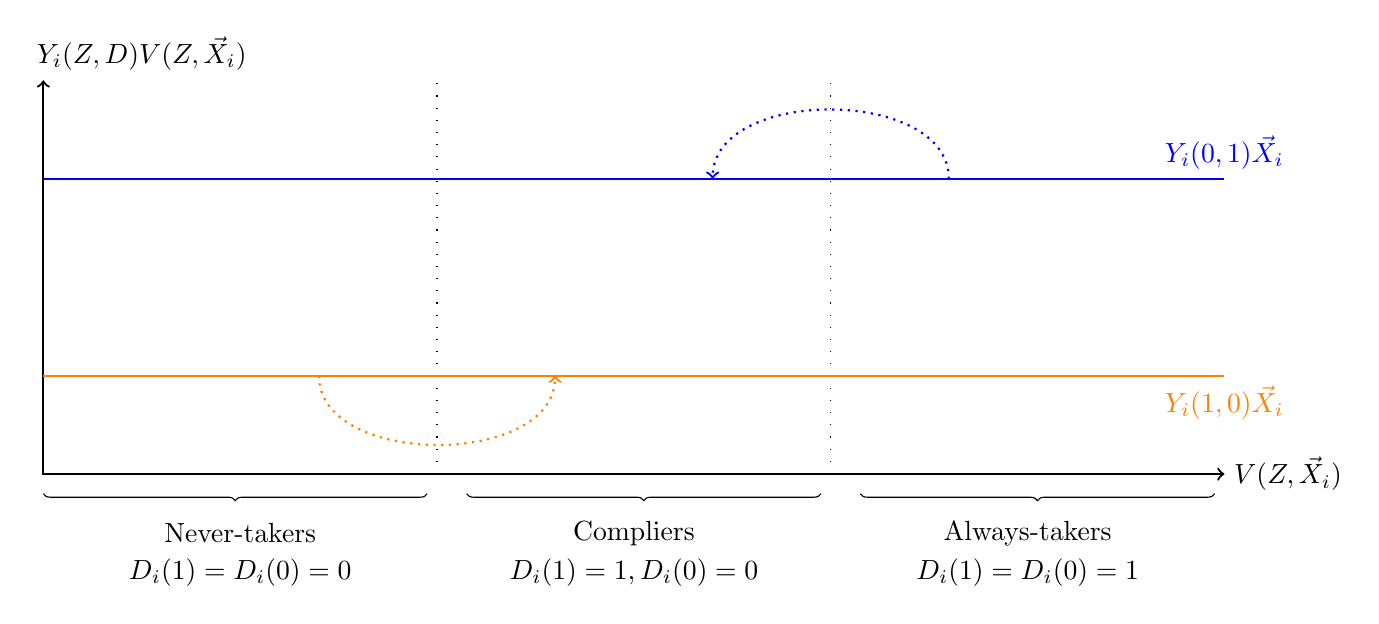
\begin{tikzpicture}[scale=5]
        % Axis
        \draw[thick,<->] (0,1)--(0,0)--(3,0);
        % Labels
        \node [above] at (0.25,1) {$\Egiven{Y_i(Z,D)}{V(Z, \vec{X}_i)}$};
        \node [right] at (3,0) {$V(Z, \vec{X}_i)$};
        % Draw the compliance regions
        \draw[decorate, decoration = {brace}] (0.975,-0.05) --  (0,-0.05);
        \node at (0.5,-0.15) {Never-takers};
        \node at (0.5,-0.25) {$D_i(1)=D_i(0)=0$};
        \draw[loosely dotted] (1,0)--(1,1);
        \draw[decorate, decoration = {brace}] (1.975,-0.05) --  (1.075,-0.05);
        \node at (1.5,-0.15) {Compliers};
        \node at (1.5,-0.25) {$D_i(1)=1, D_i(0)=0$};
        \draw[loosely dotted] (2,0)--(2,1);
        \draw[decorate, decoration = {brace}] (2.975,-0.05) --  (2.075,-0.05);
        \node  at (2.5,-0.15) {Always-takers};
        \node  at (2.5,-0.25) {$D_i(1)=D_i(0)=1$};
        % Draw Y_i(0, 1)
        \draw[thick,blue] (0,0.75)--(3,0.75);
        \node [above,blue] at (3,0.75) {$\Egiven{Y_i(0,1)}{\vec{X}_i}$};
        % Draw extrapolation of Y_i(0, 1)
        \draw[thick,dotted,->,blue] (2.3,0.75) to [out=90,in=90] (1.7,0.75);
        % Draw Y_i(0, 1)
        \draw[thick,orange] (0,0.25)--(3,0.25);
        \node [below,orange] at (3,0.25) {$\Egiven{Y_i(1,0)}{\vec{X}_i}$};
        % Draw extrapolation of Y_i(1, 1)
        \draw[thick,dotted,->,orange] (0.7,0.25) to [out=-90,in=-90] (1.3,0.25);
    \end{tikzpicture}
    \justify
    \footnotesize
    \textbf{Note}:
    The figure shows how the CCI assumption \ref{assumption:compliance-ignorability} works.
    The $x$-axis partitions compliers from non-compliers --- i.e., $V(.;.)$ is the theoretical latent-index implied by the IV assumptions \citep{vytlacil2002independence}. 
    The dotted blue arrow represents that $\Egiven{Y_i(0,1)}{\vec{X}_i}$ can be extrapolated out of the always-takers group to compliers.
    The dotted orange arrow represents that $\Egiven{Y_i(1,0)}{\vec{X}_i}$ can be extrapolated out of the never-takers group to compliers.
\end{figure}

This allows for extrapolation of conditional average earnings across compliance groups.
$Y_i(0, 1)$ is only observed among always--takers, so to identify the unconditional expectation, we must extrapolate $\Egiven{Y_i(0,1)}{\vec X_i}$ from $\vec X_i$ values for those with $Z_i = 0, D_i = 1$ to all values of $\vec X_i$.
\autoref{fig:ignorability-compliance-extrapolate} shows this assumption for $\Egiven{Y_i(0,1)}{\vec X_i}$, and \autoref{fig:ignorability-compliance-sum} the corresponding for $\Egiven{Y_i(1,1)}{\vec X_i}$.

\begin{figure}[h!]
    \centering
    \caption{Conditional Compliance Ignorability (CCI) Across Compliance Regions.}
    \label{fig:ignorability-compliance-sum}
    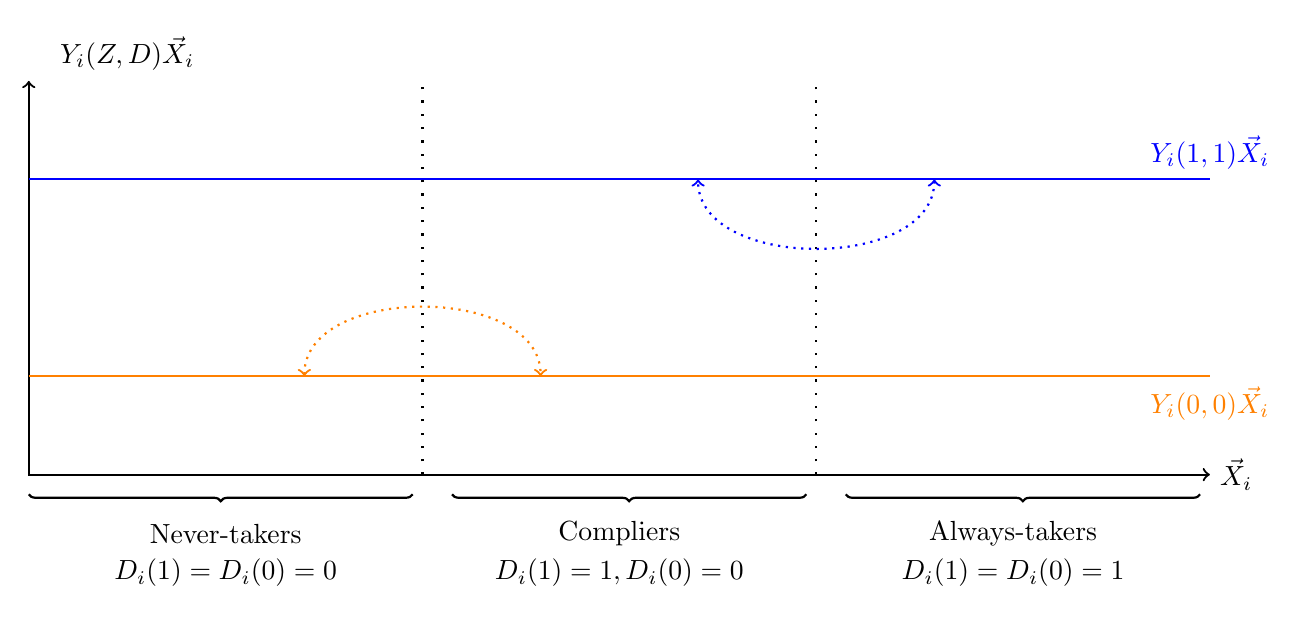
\begin{tikzpicture}[thick,scale=5]
        % Axis
        \draw[thick,<->] (0,1)--(0,0)--(3,0);
        % Labels
        \node [above] at (0.25,1) {$\Egiven{Y_i(Z,D)}{\vec{X}_i}$};
        \node [right] at (3,0) {$\vec{X}_i$};
        % Draw the compliance regions
        \draw[decorate, decoration = {brace}] (0.975,-0.05) --  (0,-0.05);
        \node at (0.5,-0.15) {Never-takers};
        \node at (0.5,-0.25) {$D_i(1)=D_i(0)=0$};
        \draw[loosely dotted] (1,0)--(1,1);
        \draw[decorate, decoration = {brace}] (1.975,-0.05) --  (1.075,-0.05);
        \node at (1.5,-0.15) {Compliers};
        \node at (1.5,-0.25) {$D_i(1)=1, D_i(0)=0$};
        \draw[loosely dotted] (2,0)--(2,1);
        \draw[decorate, decoration = {brace}] (2.975,-0.05) --  (2.075,-0.05);
        \node  at (2.5,-0.15) {Always-takers};
        \node  at (2.5,-0.25) {$D_i(1)=D_i(0)=1$};
        % Draw Y_i(1, 1)
        \draw[thick,blue] (0,0.75)--(3,0.75);
        \node [above,blue] at (3,0.75) {$\Egiven{Y_i(1,1)}{\vec{X}_i}$};
        % Draw extrapolation of Y_i(1, 1)
        \draw[thick,dotted,<->,blue] (2.3,0.75) to [out=-90,in=-90] (1.7,0.75);
        % Draw Y_i(0, 0)
        \draw[thick,orange] (0,0.25)--(3,0.25);
        \node [below,orange] at (3,0.25) {$\Egiven{Y_i(0,0)}{\vec{X}_i}$};
        % Draw extrapolation of Y_i(0, 0)
        \draw[thick,dotted,<->,orange] (0.7,0.25) to [out=90,in=90] (1.3,0.25);
    \end{tikzpicture}
    \justify
    \footnotesize
    \textbf{Note}:
    The figure shows how the CCI assumption \ref{assumption:compliance-ignorability} works.
    The dotted blue arrow represents that $\Egiven{Y_i(1,1)}{\vec{X}_i}$ is observed as the sum of outcomes among the always-takers and compliers.
    The dotted orange arrow represents that $\Egiven{Y_i(1,0)}{\vec{X}_i}$ is observed as the sum of outcomes among the always-takers and compliers.
\end{figure}

Under the CCI assumption, the conditional mechanism effect is identified.
\begin{align*}
    & \Egiven{ Z_i \left(Y_i(1, 1) - Y_i(1, 0) \right)
    + (1 - Z_i) \left(Y_i(0, 1) - Y_i(0, 0) \right)}{\vec X_i} \\
    =& \Probgiven{Z_i = 1}{\vec X_i} \left(
        \Egiven{ Y_i }{ \vec X_i, Z_i = D_i = 1}
            - \Egiven{ Y_i }{ \vec X_i, Z_i = 1, D_i = 0} \right) \\
    &+ \Probgiven{Z_i = 0}{\vec X_i} \left(
        \Egiven{ Y_i }{ \vec X_i, Z_i = 0, D_i = 1}
            - \Egiven{ Y_i }{ \vec X_i, Z_i = D_i = 0} \right)
\end{align*}
The unconditional average mechanism effect comes from integrating across the entire distribution $\vec X_i$ \citep{frolich2007nonparametric}, giving a matching--type identification.
\begin{align*}
    & \E{ Y_i(., 1) - Y_i(., 0) } \\
    &=\E[\vec X_i]{ \Egiven{ Y_i(., 1) - Y_i(., 0) }{\vec X_i}} \\
    &= \E[\vec X_i]{ \Egiven{ Z_i \left(Y_i(1, 1) - Y_i(1, 0) \right)
    + (1 - Z_i) \left(Y_i(0, 1) - Y_i(0, 0) \right)}{\vec X_i}} \\
    &= \Prob{Z_i = 1} \E[\vec X_i]{
        \Egiven{ Y_i }{ \vec X_i, Z_i = D_i = 1}
            - \Egiven{ Y_i }{ \vec X_i, Z_i = 1, D_i = 0} } \\
    &\;\;\;\; + \Prob{Z_i = 0} \E[\vec X_i]{
        \Egiven{ Y_i }{ \vec X_i, Z_i = 0, D_i = 1}
            - \Egiven{ Y_i }{ \vec X_i, Z_i = D_i = 0}}
\end{align*}

The equation for average direct effect is less simple, since $D_i$ is not independent of potential outcomes $Y_i(Z, D)$.
To get around this, exploit the fact that the total effect is the sum of direct effect and mechanism effect (times first-stage).
\begin{align*}
    & \Egiven{ D_i \left(Y_i(1, 1) - Y_i(1, 0) \right)
    + (1 - D_i) \left(Y_i(0, 1) - Y_i(0, 0) \right)}{\vec X_i} \\
    &= \bigl( \Egiven{Y_i}{\vec X_i, Z_i = 1} -
        \Egiven{Y_i}{\vec X_i, Z_i = 0} \bigr) \\
    & \;\;\;\; -
    \bigl( \Egiven{D_i}{ \vec X_i, Z_i = 1} - \Egiven{D_i}{ \vec X_i, Z_i = 0}
        \bigr) \times \\
    & \;\;\;\; \;\;\;\; \;\;
    \Egiven{ Z_i \left(Y_i(1, 1) - Y_i(1, 0) \right)
            + (1 - Z_i) \left(Y_i(0, 1) - Y_i(0, 0) \right)}{\vec X_i}
\end{align*}

\subsection{Equivalence Between SI and CCI}
\begin{proof}[Proof of~\autoref{theorem:cci-si}]
    \label{proof:cci-si}
    \textbf{Proof equating SI and CCI.}
\end{proof}

\subsection{Partial Identification}
\label{sec:partial}

CCI is a very strong assumption.
It means that characteristics $\vec X_i$ fully explains later-life earning differences between compliers and always-/never-attenders;
there are no unobserved characteristics which could explain mean differences.
This assumes that in the HRS sample all the characteristics in \autoref{tab:hrs-summary} explain mean differences between higher education compliers, and non-compliers.
This could be broken if, for example, parents' social economic status (beyond level of education) is a factor which affects their children's earnings, but is not directly observed in these data.
Children of parents of higher social class often place into higher paying, professional jobs, regardless of whether they are predisposed to, or attend, higher education.
So that it is likely that the CCI assumption does not hold exactly for selection into higher education;
\autoref{sec:plausibility} presents the formal model for how CCI rules out \cite{roy1951some} style selection into treatment based on unobserved factors.

The partially identified bounds on the AME parameter correspond to the case that CCI is broken to a plausible extent.\footnote{
    Note that the approach here is similar to that by \cite{flores2013partial}, but bounds a different theoretical parameter.
    \cite{flores2013partial} develop Lee-type bounds for one side of the AME local to compliers i.e., bounds for $\Egiven{Y_i(Z_i, 1) - Y_i(Z_i, 0)}{Z_i =1, D_i(1)=1, D_i(0) = 0}$.
    Also note that the approach here bounds the AME (and not the LAME for compliers), as AME bounds are tighter than those for subgroups without the exclusion restriction.
}
The bounds here require a weaker assumption than CCI.
\begin{assumption}
    \label{assumption:compliance-monotonicity}
    Conditional Compliance Monotonicity (CCM) with respect to $Z_i$.
    \begin{enumerate}
        \item \label{assumption:compliance-monotonicity-POs}
        $\Egiven{Y_i(z, d)}{\vec X_i, D_i(1) = D_i(0) = 0}
        \leq \Egiven{Y_i(z, d)}{\vec X_i, D_i(1) = 1, D_i(0) = 0}$ \\
        $\leq \Egiven{Y_i(z, d)}{\vec X_i, D_i(1) = D_i(0) = 1}$
        almost surely, for $z, d = 0, 1$.
        \item \label{assumption:compliance-monotonicity-z}
        $\Egiven{Y_i(1,0)}{\vec X_i, D_i(1) = 1}
        \leq \Egiven{Y_i}{\vec X_i, Z_i = 1}$, and
        $\Egiven{Y_i}{\vec X_i, Z_i = 0}
        \leq \Egiven{Y_i(0,1)}{\vec X_i, D_i(0) = 0}$.
    \end{enumerate}
\end{assumption}
CCM assumes that earnings for compliance groups have the following average order (lowest to highest): never--takers, compliers, always--takers.
This is rationalisable in a Roy-style selection into treatment framework:
never--takers choose not to attend higher education as they would have the lowest earnings gain from attending, while compliers have an earnings increase if they have the higher EA score, and always--takers always select into higher education.
The second part is an assumption that the violation of the exclusion restriction operates in the same direction as treatment.
Here, this means a higher EA Score $Z_i = 1$ leads to higher earnings, in the same way that attending higher education $D_i = 1$ leads to higher earnings.

Under the CCM assumption \ref{assumption:compliance-monotonicity}, the AME has following bounds --- where the CCI point estimate above is the upper bound.
\begin{align*}
    & \Probgiven{Z_i = 1}{\vec X_i} \Probgiven{D_i(1) = 1}{\vec X_i} \left(
        \Egiven{ Y_i }{ \vec X_i, Z_i = D_i = 1}
            - \Egiven{ Y_i }{ \vec X_i, Z_i = 1} \right) \\
    &+ \Probgiven{Z_i = 0}{\vec X_i} \Probgiven{D_i(0) = 0}{\vec X_i} \left(
        \Egiven{ Y_i }{ \vec X_i, Z_i = 0}
            - \Egiven{ Y_i }{ \vec X_i, Z_i = D_i = 0} \right) \\
    \leq & \Egiven{ Z_i \left(Y_i(1, 1) - Y_i(1, 0) \right)
    + (1 - Z_i) \left(Y_i(0, 1) - Y_i(0, 0) \right)}{\vec X_i} \\
    \leq& \Probgiven{Z_i = 1}{\vec X_i} \left(
        \Egiven{ Y_i }{ \vec X_i, Z_i = D_i = 1}
            - \Egiven{ Y_i }{ \vec X_i, Z_i = 1, D_i = 0} \right) \\
    &+ \Probgiven{Z_i = 0}{\vec X_i} \left(
        \Egiven{ Y_i }{ \vec X_i, Z_i = 0, D_i = 1}
            - \Egiven{ Y_i }{ \vec X_i, Z_i = D_i = 0} \right)
\end{align*}
\textbf{Proof:} See \autoref{sec:ame-bounds}.


\subsection{Estimation}
\label{sec:estimation}

The primary estimation step involves estimating multiple conditional expectations;
the prediction and extrapolation steps are carried out in the following manner.
% \textbf{To-do: Write the adjusted causal forest approach, and estimate on HRS data.}

\begin{enumerate}
    \item Estimate $\Egiven{ Y_i }{ \vec X_i, Z_i, D_i}$.
    In principle this step can involve any regression approach; I use honest regression forests to allow for non-linearities between $Y_i, \vec X_i, Z_i, D_i$, and to automate cross-fitting to avoid within sample over-fitting \citep{athey2019generalized}.
    Predict values $\hat{Y_i(1,1)} = \hat{\Egiven{ Y_i }{ \vec X_i, Z_i = D_i = 1}}$ across the entire sample.
    \item Repeat the process for $\hat{Y_i(0,1)}, \hat{Y_i(1,0)}, \hat{Y_i(0,0)}$. %, and for compliance scores.
    \item Calculate the average effects as the mean of relevant predictions:
    \[ \hat{\text{AME}}
    = \frac 1n \sum_{i=1}^N \left[ 
        \hat{\Probgiven{Z_i = 1}{\vec X_i}} \left( \hat{ Y_i(1,1)} - \hat{Y_i(1, 0)} \right)
        + \hat{\Probgiven{Z_i = 0}{\vec X_i}} \left( \hat{ Y_i(0,1)} - \hat{Y_i(0, 0)} \right) \right]
    \]
    \item Calculate the compliance scores, and $\hat{\Egiven{Y_i}{\vec X_i, Z_i}}$ by the same process, to give the partially identified bounds.
\end{enumerate}

Given the nested prediction exercise, estimation and sampling error both play a role in estimate inference.
Standard errors can be computed via bootstrap sampling.

\subsection{Plausibility of CCI}
\label{sec:plausibility}

The above develops point identification under the CCI assumption.
This approach corresponds to assuming no sorting into $D_i$ on unobservables, explcuding a primary motivation for IV-type empirical strategies.
This section formalises how CCI implies no sorting on unobservables, following an explanation by \cite{angrist2010extrapolate}, but now does not assume the exclusion restriction holds.

Assuming CCI--- that average POs do not vary except via characteristics $\vec X_i$ --- is a strong assumption.
Notably, CCI does not apply in the presence of \cite{roy1951some} style selection on treatment gains from unobserved factors.\footnote{
    This explanation follows the approach shown by \cite{angrist2010extrapolate}, but now does not assume the exclusion restriction holds.
}
To formalise this statement, consider a Roy style model for selection into treatment, where POs vary by characteristics and instrument via $f_D(.;.)$ and independent unobserved (mean zero) factors $\varepsilon_D$.
\[ Y_i(Z, 1) = f_1(\vec X_i ; Z) + \varepsilon_1, \;\;
    Y_i(Z, 0) = f_0(\vec X_i ; Z) + \varepsilon_0
        \text{, for Z} = 0,1 \]
\cite{vytlacil2002independence} shows that the latent index model for selection is implied by the LATE assumptions.
Write $f(.;.)$ for the implied index function, representing the sum of treatment benefits and costs implied by characteristics and instrument receipt.
\[ D_i(Z) = \indicator{f(\vec X_i; Z) \geq 0} \]
Roy style selection based on treatment gains would have the latent index as whether selection into treatment is a net gain to the individual: $f(\vec X_i ; Z) = \left( f_1(\vec X_i; Z) - f_0(\vec X_i; Z)\right) +
\left( \varepsilon_1 - \varepsilon_0 \right)$.

Now consider POs for the compliers.
\begin{align*}
    &\Egiven{Y_i(Z,D)}{\vec X_i, D_i(1)=1, D_i(0)=0} \\
    &= \Egiven{f_D(\vec X_i ; Z) + \varepsilon_D}{\vec X_i,
        f_1(\vec X_i; 1) + \varepsilon_1 \geq 0 \geq f_0(\vec X_i; 0) + \varepsilon_0} \\
        &= f_D(\vec X_i ; Z) + \Egiven{\varepsilon_D}{\vec X_i,
            f_1(\vec X_i; 1) + \varepsilon_1 \geq 0 \geq f_0(\vec X_i; 0) + \varepsilon_0}
\end{align*}
So that Roy style selection into treatment has POs positively correlated with idiosyncratic factors $\varepsilon_1, \varepsilon_0$.

Compare with the CCI assumption, which has POs equal across compliance groups:
\begin{align*}
    &\Egiven{Y_i(Z,D)}{\vec X_i, D_i(1)=1, D_i(0)=0}
    = \Egiven{Y_i(Z,D)}{\vec X_i} \\
    \implies&
        \Egiven{f_D(\vec X_i ; Z) + \varepsilon_D}{\vec X_i,
            D_i(1)=1, D_i(0)=0} \\
    &= f_D(\vec X_i ; Z) + \Egiven{\varepsilon_D}{\vec X_i,
        D_i(1)=1, D_i(0)=0} \\
    &= f_D(\vec X_i ; Z) + \Egiven{\varepsilon_D}{\vec X_i} \\
    &= f_D(\vec X_i ; Z) \\
    \implies& \varepsilon_1, \varepsilon_0 \perp D_i(1), D_i(0)
\end{align*}
So CCI is only credible if positive selection into treatment involves only mean-independent unobserved factors $\varepsilon_1, \varepsilon_0$, and mean-dependence is captured fully by observed characteristics $\vec X_i$.

\subsection{AME Bounds}
\label{sec:ame-bounds}

Under CCM, the AME has sharp bounds.
To show this, start by bounding $\Egiven{Y_i(1,1)}{\vec X_i}$.

First, see that $\Egiven{Y_i(1,1)}{\vec X_i}$ is the sum of one observed expectation and another which can be bounded.
\begin{align*}
    &\Egiven{Y_i(1,1)}{\vec X_i} \\
    &=
    \Probgiven{D_i(1) = 1}{\vec X_i }
        \Egiven{Y_i(1,1)}{\vec X_i, D_i(1) = 1}
    + \Probgiven{D_i(1) = 0}{\vec X_i }
        \Egiven{Y_i(1,1)}{\vec X_i, D_i(1) = 0} \\
    &=
    \Probgiven{D_i(1) = 1}{\vec X_i }
        \Egiven{Y_i}{\vec X_i, Z_i = D_i = 1}
    + \Probgiven{D_i(1) = 0}{\vec X_i }
        \Egiven{Y_i(1,1)}{\vec X_i, D_i(1) = D_i(0) = 0}
\end{align*}

$\Egiven{Y_i(1,1)}{\vec X_i, D_i(1) = D_i(0) = 0}$ is the PO for never-takers, so by the CCM assumption has following bounds.
\[
    \Egiven{Y_i}{\vec X_i, Z_i = 1} 
    \leq 
    \Egiven{Y_i(1,1)}{\vec X_i, D_i(1) = D_i(0) = 0} 
    \leq 
    \Egiven{Y_i}{\vec X_i, Z_i = 1, D_i = 1}
\]

Exploit the same process for $\Egiven{Y_i(1,0)}{\vec X_i}$.
\begin{align*}
    &\Egiven{Y_i(1,0)}{\vec X_i} \\
    &=
    \Probgiven{D_i(1) = 1}{\vec X_i }
        \Egiven{Y_i(1,0)}{\vec X_i, D_i(1) = 1}
    + \Probgiven{D_i(1) = 0}{\vec X_i }
        \Egiven{Y_i(1,0)}{\vec X_i, D_i(1) = 0} \\
    &=
    \Probgiven{D_i(1) = 1}{\vec X_i }
        \Egiven{Y_i(1,0)}{\vec X_i, D_i(1) = 1}
    + \Probgiven{D_i(1) = 0}{\vec X_i }
        \Egiven{Y_i}{\vec X_i, Z_i = 1, D_i = 0}
\end{align*}
$\Egiven{Y_i(1,0)}{\vec X_i, D_i(1) = 1}$ is the pooled PO for always-takers and compliers, so by the CCM assumption has following bounds.
\[
    \Egiven{Y_i}{\vec X_i, Z_i = 1, D_i = 0}
    \leq 
    \Egiven{Y_i(1,0)}{\vec X_i, D_i(1) = 1} 
    \leq 
    \Egiven{Y_i}{\vec X_i, Z_i = 1}
\]

And so that the first part of the AME has the following bounds.
\begin{align*}
    &\Probgiven{D_i(1) = 1}{\vec X_i } \big( 
        \Egiven{Y_i}{\vec X_i, Z_i = 1, D_i = 1}
        - \Egiven{Y_i}{\vec X_i, Z_i = 1}
    \big) \\
    &\leq
    \Egiven{Y_i(1,1) - Y_i(1,0)}{\vec X_i} \\
    &\leq
    \Egiven{Y_i}{\vec X_i, Z_i = D_i = 1}
        - \Egiven{Y_i}{\vec X_i, Z_i = 1, D_i = 0}
\end{align*}

The exact same reasoning leads to bounds for the other side.
\begin{align*}
    &\Probgiven{D_i(0) = 0}{\vec X_i } \big( 
        \Egiven{Y_i}{\vec X_i, Z_i = 0}
        - \Egiven{Y_i}{\vec X_i, Z_i = D_i = 0}
    \big) \\
    &\leq
    \Egiven{Y_i(0,1) - Y_i(0,0)}{\vec X_i} \\
    &\leq
    \Egiven{Y_i}{\vec X_i, Z_i = 0, D_i = 1}
        - \Egiven{Y_i}{\vec X_i, Z_i = 0, D_i = 0}
\end{align*}
And finally, the AME bounds are composed between these.
